
\section{The Infomax Principle}

\mode<presentation>{
\begin{frame} 
    \begin{center} \huge
        \secname \\
        (Bell \& Sejnowski, 1995)
    \end{center}
    \begin{center}
    Applying Information theory + density transformation to solve the ICA problem.
    \end{center}
\end{frame}
}

\begin{frame}{The Infomax Principle (Bell \& Sejnowski, 1995)}

\begin{itemize}
\item[\emph{Idea:}] Under certain conditions, maximizing the
  \emph{mutual information} between inputs (mixed signals $\vec x$) and outputs
  (recovered sources $\widehat{\vec s}$) of a system yields \emph{independent} outputs.\\
  
  \svspace{5mm}
  
\item[]
  If sources are independent, then
  transformations of these sources are independent, too.\\
  
  \svspace{5mm}
  
\item[]  
  Choosing the transformation such that their marginal distributions become uniform 
  simplifies the computations to find independent sources. i.e. choosing the transformation \\
  
\begin{equation}
\widehat{u}_i = \widehat{f}_i(\widehat{s}_i)
\quad \text{such that} \quad
\widehat{P}_{u_i}(\widehat{u}_i) = \mathrm{const.}
\label{eq:transfconst}
\end{equation}

\end{itemize}

\end{frame}

\subsubsection{Putting Infomax and density transformation together}

\begin{frame}{\subsubsecname}

\notesonly{\underline{Recap on Density Transformation}:\\}

The transformation is found using \emph{conservation of probability}
\begin{equation}
	\widehat{P}_{u_i}(\widehat{u}_i) d \widehat{u}_i 
	\; =  \; \widehat{P}_{s_i} (\widehat{s}_i) d \widehat{s}_i.
\end{equation}
for marginals, and
\begin{equation}
	\widehat{P}_{\vec u}(\widehat{\vec u}) d \widehat{\vec u} 
	\; =  \; \widehat{P}_{\vec s} (\widehat{\vec s}) d \widehat{\vec s}.
\end{equation}
for the joint distribution.


Using the general rule for density transformations and applying it here yields
\begin{equation}
\label{eq:conservation1}
	\widehat{P}_{u_i}(\widehat{u}_i) \quad
	 =  \quad \bigg| 
		\frac{d \widehat{s}_i}{d \widehat{u}_i} \bigg| 
			 \widehat{P}_{s_i}(\widehat{s}_i) \quad
	 =  \quad \frac{1}{\big| \widehat{f}_i^{'} (\widehat{s}_i) \big|} 
		\widehat{P}_{s_i}(\widehat{s}_i)
\end{equation}
where $\left|\frac{d \widehat{s}_i}{d \widehat{u}_i} \right|$ is
called \emph{functional determinant} of the transformation
$\widehat{f}_i$.

Analogously for the joint distribution:
\begin{equation}
\label{eq:conservation1joint}
	\widehat{P}_{\vec u}(\widehat{\vec u}) \quad
	 =  \quad \bigg| 
		\frac{d \widehat{\vec s}}{d \widehat{\vec u}} \bigg| 
			 \widehat{P}_{\vec s}(\widehat{\vec s})
\end{equation}

\end{frame}

\begin{frame}{Putting Infomax and density transformation together}


\question{What kind of transformation does Infomax need?}

\pause

Infomax requires a transformation resulting in a uniformly distributed
variable with a constant density\notesonly{ (cf. \eqref{eq:transfconst}}.

\slidesonly{
\begin{equation}\widehat{u}_i = \widehat{f}_i(\widehat{s}_i) 
\quad st. \quad
\widehat{P}_{u_i}(\widehat{u}_i) = \mathrm{const.}
\end{equation}
}

\question{What is the density transformation for? }

\pause

-conservation of probability

\end{frame}

\begin{frame}{Putting Infomax and density transformation together}

\svspace{-5mm}

\notesonly{This yields:}

\begin{equation}
  \label{eq:dtufs}
		\widehat{P}_{u_i} (\widehat{u}_i) \; = \;   
		 \frac{1}{\big| \widehat{f}_i^{'} (\widehat{s}_i) \big|} 
		\widehat{P}_{s_i}(\widehat{s}_i) \; \stackrel{!}{=} \; \text{const.} \quad \Rightarrow \quad 
		 \big| \widehat{f}_i^{'} (\widehat{s}_i) \big| =  a \widehat{P}_{s_i}(\widehat{s}_i) 
\end{equation}
and therefore

\svspace{-3mm}

\begin{equation}
\Rightarrow \widehat{f}_i (\widehat{s}_i)
 = \int\limits_{-\infty}^{\widehat{s}_i} dy\; a 
			\widehat{P}_{s_i}(y)
\end{equation}

\begin{figure}[h]
  \centering
  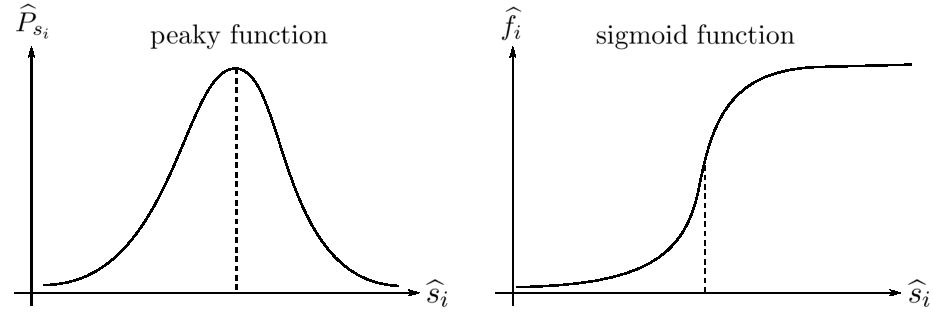
\includegraphics[width=0.7\textwidth]{img/section2_fig15}  
  %\caption{density (pdf) and corresponding distribution function (cdf)}
  \label{fig:cdf}
\end{figure}

\svspace{-2mm}

\question{Why didn't we use the Inverse CDF technique?}

\notesonly{
We don't have an expression for the pdf of the variables to formulate the inverse of its cdf.
}

\end{frame}

\newpage

\begin{frame}{Two Equivalent Approaches to formulating the cost function for Infomax}

\pause

\only<2>{
\slidesonly{
\begin{center}
	
\includegraphics[width=0.4\textwidth]{img/meme_morethanone}
\end{center}
}
}

\slidesonly{
\begin{enumerate}
\item Maximizing mutual information directly - overview only

\pause

\slidesonly{
\begin{center}
	
\includegraphics[width=0.3\textwidth]{img/meme_infomaxisabout}
\end{center}
}

\item Infomax via KL-divergence for the transformed densities
\end{enumerate}


}


\end{frame}

\section{Approach 0: Maximizing mutual information directly - overview only}

\begin{frame}

\notesonly{
One way to formulate the cost function for the Infomax algorithm is to maximize the mutual information directly:
}

\begin{equation}
I(Y,X) = h(Y) - h(Y|X)
\end{equation}

\notesonly{By considering}\slidesonly{Consider} the following relationship between $Y$ and $X$:\\
$Y = g(X;w) + \mathcal{N}$, where $g(\cdot)$ is some invertible transformation parametrized by $w$ and $\mathcal{N}$ is additive noise.

By taking the derivative with respect to the parameter $w$:

\begin{equation}
\frac{\partial}{\partial w} I(Y,X) = \frac{\partial}{\partial w}h(y) - 
\underbrace{\frac{\partial}{\partial w} h(Y|X)}_{= \frac{\partial}{\partial w} h(\mathcal{N}) = 0}
\end{equation}

Maximizing $I(Y,X)$ boils down to maximizing the (differential) entropy of the output $Y$. 

%\notesonly{
%We've seen how mutual information relates to the KL divergence, so we're going to use an approach 
%that operates on the KL-divergence. 
%Whether Infomax by maximizing entropy\footnote{if interested see Bell, A. J., \& Sejnowski, T. J. (1995). An information-maximization approach to blind separation and blind deconvolution. Neural computation, 7(6), 1129-1159.} 
%or finding a factorization via the KL-divergence,
%both are based on the Infomax principle and arrive at the same solution.
%}

\end{frame}

\clearpage

\section{Approach 1: Infomax via KL-divergence for the transformed densities}

\begin{frame}{\secname}

\slidesonly{
\visible<2->{
\vspace{-14mm}
\hspace{8.0cm}
\StickyNote[1.7cm]{
	\begingroup
	\scriptsize
	%\begin{equation}
		%\widehat{P}_{u_i} (\widehat{u}_i) =
		 %\frac{1}{\big| \widehat{f}_i^{'} (\widehat{s}_i) \big|} 
		 %\widehat{P}_{s_i}(\widehat{s}_i)
	%\end{equation}
	\begin{equation}
	{P}_{\vec u}(\widehat{\vec u}) d \widehat{\vec u} 
	\; =  \; {P}_{\vec s} (\widehat{\vec s}) d \widehat{\vec s}
	\end{equation}
\vspace{-2mm}
	\begin{equation}
\label{eq:conservation1joint}
	{P}_{\vec u}(\widehat{\vec u}) \;
	 =  \; \bigg| 
		\frac{d \widehat{\vec s}}{d \widehat{\vec u}} \bigg| 
			 {P}_{\vec s}(\widehat{\vec s})
\end{equation}
\vspace{-2mm}
	\begin{equation}
		\widehat{P}_{u_i}(\widehat{u}_i) := \; \text{const}
	\end{equation}
	\endgroup
}[3.cm] % width
\vspace{-22mm}
}
}

\slidesonly{
\begingroup
\small
}
\begin{align}
  \dkl 
  & = \int d \, \widehat{\vec{s}} P_{\vec{s}}(\widehat{\vec{s}}) \ln \frac{P_{\vec{s}}(\widehat{\vec{s}})}{\prod_i \widehat{P}_{s_i}(\widehat{s}_i)} \slidesonly{\hspace{35mm}}\\
\notesonly{  \intertext{Using the factorization in \eqref{eq:facts}:}}
\visible<2->{
  & = \int d \, \widehat{\vec{s}} P_{\vec{s}}(\widehat{\vec{s}}) \ln \frac{P_{\vec{s}}(\widehat{\vec{s}})}{\widehat{P}_{\vec{s}}(\widehat{\vec{s}})}
\slidesonly{\\}
\notesonly{  \intertext{Applying the density transformation:} }
  %& = &  \int d \, \widehat{\vec{s}} P_{\vec{s}}(\widehat{\vec{s}}) \ln 
  %\frac
  %{P_{\vec{s}}(\widehat{\vec{s}}) \quad \prod_i \frac{1}{f_i' (\widehat{s}_i)}}
  %{\prod_i \widehat{P}_{s_i}(\widehat{s}_i) \quad \frac{1}{f_i' (\widehat{s}_i)}} \\
    %\pause
  & = \int d \, \widehat{\vec{s}} P_{\vec{s}}(\widehat{\vec{s}}) \ln 
  \frac
  {
  \Big|  \frac{d \widehat{\vec u}}{d \widehat{\vec s}} \Big|
  {P}_{\vec u}(\widehat{\vec u}) 
  }
  {
    \Big|  \frac{d \widehat{\vec u}}{d \widehat{\vec s}} \Big|
  \widehat{P}_{\vec u}(\widehat{\vec u}) 
  }
}
\visible<3->{
\slidesonly{\\}
\notesonly{  \intertext{The same factorization in \eqref{eq:facts} equally applies to the transformed variables $\vec u$:} }
  & = \int d \widehat{\vec{u}} P_{\vec{u}} (\widehat{\vec{u}}) 
  \ln 
  \frac
  {P_{\vec{u}} (\widehat{\vec{u}}) }
  {\prod_i  \widehat{P}_{u_i}(\widehat{u_i})} \\
  & = 
  \underbrace{
	  \int d \widehat{\vec{u}} P_{\vec{u}} (\widehat{\vec{u}}) 
	  \ln 
	  {P_{\vec{u}} (\widehat{\vec{u}}) }
  }_{= -H \; \text{(negative entropy)}}\notesonly{\\
  & \quad -}\slidesonly{\;\; - \;\;}
  \underbrace{
	  \int d \widehat{\vec{u}} P_{\vec{u}} (\widehat{\vec{u}}) 
	  \bigg( \ln
	  {\prod_{i=1}^{N}
	  \overbrace{ 
		\widehat{P}_{u_i}(\widehat{u_i}) 
	  }^{\substack{\text{const.\;}\notesonly{ a \\\text{\;see \eqref{eq:dtufs}}}}}} 
	  \bigg)
	  }_{\text{constant}}
}
\end{align}
\slidesonly{
\endgroup
}

\end{frame}



\begin{frame}

This gives us a new but equivalent formulation for the Infomax optimization problem:
\begin{equation}\label{eq:infomax}
  H = -\int d \widehat{\vec{u}} P_{\vec{u}} (\widehat{\vec{u}})
  \ln P_{\vec{u}} (\widehat{\vec{u}}) \eqexcl \max_{\vec W} 
\end{equation}

using the transformed estimated sources
\begin{equation}
\widehat{u}_i := \widehat{f}_i \big( \underbrace{ \vec{e}_i^\top
		\vec{W} \, \vec{x}  }_{= \widehat{s_i} } \big) 
\end{equation}

where $\vec e_i$ is a \emph{basis} vector where the $i$-th element is equal to 1 and all other elements are zero.
Example for $\vec e_i$ for selecting the $i$-th reconstruction with 2D observations:
\begin{equation}
\textcolor{blue}{\hat {\mathrm{s}}_2} =
\overbrace{
\big( \, 0 \;\; \textcolor{blue}{1} \, \big) 
}^{\vec e_2^\top}
	\left( \begin{array}{ll}
	{\mathrm{w}_{11}} & {\mathrm{w}_{12}} \\
		{\mathrm{w}_{21}} & {\mathrm{w}_{22}} 
	\end{array} \right)
	\left( \begin{array}{ll}
		\mathrm{x}_1 \\ \mathrm{x}_2
	\end{array} \right)
	= \big( \, 0 \;\; \textcolor{blue}{1} \, \big)
	\left( \begin{array}{ll}
		\hat {\mathrm{s}}_1 \\ \textcolor{blue}{\hat {\mathrm{s}}_2}
	\end{array} \right)
\end{equation}

\end{frame}

\begin{frame}

\question{What does this tell us?}

\pause

This tells us that 
\begin{itemize}
\item we can produce statistically independent sources $\widehat {\vec s}$ 
by maximizing the entropy of their transformation $\vec u$.
\only<3>{
\item maximizing the entropy of $\vec u$ is equivalent minimizing \notesonly{\eqref{eq:klmin}}
}

\begingroup
\footnotesize
\begin{equation}
\label{eq:klminequivh}
\visible<2->{
 \quad H(\vec u) \eqexcl \max_{\vec W} 
 }
 \visible<3->{
  \;\; \Leftrightarrow \;\;
 	\dkl\lbrack P_{\vec{s}}(\widehat{\vec{s}}),\widehat{P}_{\vec{s}}(\widehat{\vec{s}})\rbrack = 
    \int d \, \widehat{\vec{s}} \; P_{\vec{s}}(\widehat{\vec{s}})
		\ln \frac{P_{\vec{s}}(\widehat{\vec{s}})}{
			\prod_{i = 1}^N \widehat{P}_{s_i}(\widehat{s}_i) }
		\eqexcl \min_{\vec{W}} 
 }
\end{equation}
\endgroup
\pause

\item It is equivalent to maximizing the mutual information.
Recall ``Maximizing $I(Y,X)$ boils down to maximizing the entropy of the output $Y$.''.
We now know that $Y$ is $u_i$ and $X$ is an observed variable $x_i$.

\pause

Now that we've found the cost function for our learning algorithm. 
We build something that can learn to solve the ICA problem.

\end{itemize}

\end{frame}

% -----------------------------------------------------------------------------
